\documentclass[11pt]{article}
\usepackage[margin=1in]{geometry}
\usepackage{amsmath,amssymb,amsthm}
\newtheorem{proposition}{Proposition}
\usepackage{graphicx}
\usepackage{booktabs}
\usepackage{natbib}
\usepackage{microtype}
\usepackage[hidelinks]{hyperref}
\usepackage{setspace}
\onehalfspacing

\title{Participation Gradients Discipline Coordination Traps:\\ Agency, Social Cohesion, and Activation Policy in a Heterogeneous-Agent Economy}
\author{Alessandro Conway\thanks{Draft. Companion to ``Wellbeing and the Social Fabric in a Heterogeneous-Agent Economy''; the two papers share one Julia engine, and every number and figure here is reproduced by the scripts sa\_level4.jl and sa\_figures\_l4.jl in the public repository, with the numerical checks recorded in VERIFICATION.md.}}
\date{\today}

\begin{document}
\maketitle

\begin{abstract}
\noindent I model participation in social life as a discrete choice with social interactions inside an incomplete-markets economy, in which agency, the capacity to convert effort into income, differs across education groups. The main result is a bound that turns ordinary participation statistics into a test for coordination traps. With lognormal belonging tastes, the slope of the aggregate participation map depends on the taste distribution only through its dispersion and the participation rates that distribution induces, so multiple equilibria require taste dispersion below a threshold computable from observed group rates and one preference share, with no structural estimation. The bound tightens as the participation gradient steepens: an observed education gradient is evidence against coordination traps rather than neutral with respect to them. At the French moments the bound is $0.46$ against the dispersion of $0.510$ the participation data require, so the calibrated economy sits about ten percent outside the coordination region, and the model's own numerical boundary at $0.40$ confirms the ordering. Three results follow. The education gradient in participation divides roughly two to one between the taste for belonging and agency operating through wealth, the income effect beating the price of time, which is why participation rises with income although richer households face a higher opportunity cost of time. A budget-balanced make-work-pay subsidy has a direct effect of 5.9 percentage points and an equilibrium effect of 23.9, from 35.3 percent participation to 11.3, so at this margin the complementarity amplifies policy by a factor of 4.0 at the size of shock examined, against a small-shock prediction of 8.3 from the reciprocal of one minus the very map slope the bound constrains, which ties the policy result to the theorem rather than leaving it a separate simulation. And a participation tax credit, the analogue of France's charitable-donations deduction and the United Kingdom's Gift Aid, moves participation the other way and by more, at a fraction of the fiscal cost, and remains equalising across every take-up rate examined, so two policies from the same pro-work family swap places between a GDP ledger and a GDP-B ledger.
\end{abstract}

\section{Introduction}

The companion paper to this one embeds social cohesion in a heterogeneous-agent economy and establishes two things: that a recognisable activation policy buys consumption at the cost of the social fabric, with a regressive incidence invisible to single-index evaluation, and that the smooth social-multiplier route to multiple equilibria does not survive measured labour-supply elasticities. The second finding is constructive: it says that a credible account of social coordination needs a margin whose aggregate response can be steep without an implausible intensive-margin elasticity, and the theory of social interactions has long identified that margin as a discrete choice with complementarities \citep{brock2001}. This paper builds it, and puts agency, the second SAGE dimension \citep{snower2020}, at its centre.

The discrete choice is participation in social life. One joins the association, the club, the standing commitment, or one does not; joining means committing a minimum meaningful share of time. This is not a modelling flourish but what the data measure: in the French statistical office's long-running series, 42 percent of residents belong to at least one association, the rate rises steeply with education, 56 percent above the baccalaureat against 22 percent with no diploma, and the pattern has been stable for thirty years \citep{insee2016}. Time-use data put participants' associative and social commitment at around a tenth of committed time \citep{roy2012}. The model is calibrated to exactly these moments: an aggregate participation rate of a third and group rates of one quarter and forty-five hundredths for the lower- and higher-education groups.

Four results follow.

First, and this is the paper's main contribution, the coordination question is answered with a theorem rather than a scan. In the threshold version of the model with lognormal belonging tastes, the slope of the aggregate participation map has a closed form in which the taste distribution enters only through its dispersion $\sigma_m$ and the participation rates that distribution induces. Multiple equilibria then require $\sigma_m$ to fall below a bound assembled from observed group participation rates and the private share of the participation payoff, and from nothing else: no structural estimation, no unobserved parameter. The bound has a property that gives it teeth. It is largest when groups participate at one half and shrinks as rates move apart, so the steeper the observed participation gradient, the harder coordination traps are to sustain. A visible gradient is not neutral evidence about traps; it is evidence against them. At the French moments the bound is $0.46$ while the participation data require $0.510$, so the economy sits about ten percent outside the coordination region, and because the threshold version overstates the true slope the conclusion is conservative. Scanning the full model puts its actual boundary at $0.40$, inside the analytical bound, as it must be. This is the quantitative answer to whether left-behind communities are coordination failures: in this model, disciplined by participation data, they are not. The verdict survives the one parameter the data do not pin down, the private share of the participation payoff, at every value I try; the margin does not, and at the lowest of them France sits close to the edge rather than far from it. It is also portable, because any researcher holding a participation gradient can compute the bound for their own setting.

Second, the model produces an education gradient in participation and says where it comes from. Two thirds of the gap is the taste for belonging, which the underlying wellbeing indicators put higher among the more educated. The remaining third is agency, and it works through wealth: higher agency makes households richer, richer households have a lower marginal utility of consumption, and so the fixed time commitment costs them less in utility terms. The income effect beats the price-of-time effect. This resolves, inside a structural model, the apparent puzzle of why participation rises with income although richer people face a higher opportunity cost of time, the same force that makes volunteering an increasing function of education in every survey. It also supplies the input the first result needs: the gradient is real, and it is evidence of dispersed tastes.

Third, the activation-policy result of the companion paper is sharply amplified on the participation margin, and the amplification is not a free parameter. A budget-balanced 20 percent make-work-pay subsidy raises the return to market hours and taxes everyone a lump sum to pay for it; both push against the time commitment. The direct effect, holding everyone else's participation fixed, is a fall of 5.9 percentage points. The equilibrium effect is a fall of 23.9, from 35.3 percent participation to 11.3: the social feedback multiplies the direct effect by 4.0, because each household's exit lowers the belonging return of every other household. The formula $1/(1-G')$ at the equilibrium slope predicts a multiplier of 8.3 for a small shock, so the same slope the bound of the first result constrains is the slope that sets the size of the second; the twenty-point shock examined is large enough that curvature pulls the realised multiplier below that linear prediction, and Section 6.1 reports both. A map flat enough to rule out coordination traps by only a modest margin is a map that can still amplify a large policy shock several times over, and the two statements are one statement read at two scales.

Fourth, the contrast that makes the policy point usable. Raising the lower-education group's agency to the population mean, an empowerment policy in the SAGE sense, raises equilibrium participation from 35.3 to 46.5 percent and narrows the education gap, without any fiscal instrument at all. A participation tax credit, modelled at the real rebate rates of the United Kingdom's Gift Aid and France's charitable-donations deduction, does the same from the other direction and far more cheaply: Gift Aid's 25 percent rebate lifts participation from 35.3 to 84.9 percent at a fraction of the work subsidy's fiscal cost. Because such credits are claimed unevenly, I add a take-up gradient, and the natural worry does not materialise: the credit stays equalising at every take-up rate examined. The ratio of higher- to lower-group participation is 1.65 at baseline; full take-up cuts it to 1.14, and even at a quarter take-up, where the lower group claims the rebate at only a fraction of the higher group's rate, it falls to 1.50, still below baseline. Take-up disciplines how much the credit equalises, not whether it does. Policies from the same pro-work family therefore have opposite effects on the social fabric: subsidising hours raises the price of time and unravels participation, while empowering people or paying them for the act of joining crowds it in. An evaluation framework that does not carry the social dimension cannot tell these policies apart on the margin where they differ most.

The paper proceeds as follows. Section 2 lays out the model and its relation to the shared engine. Section 3 calibrates. Section 4 presents the gradient and its decomposition, which establishes the dispersion the main result needs. Section 5 states and proves the heterogeneity-multiplicity trade-off and applies it to the French data. Section 6 runs the three policies and sets them on the two ledgers. Section 7 concludes with the welfare reading and the road to general equilibrium.

The headline calibration is for France because the supporting French data is unusually complete. The model engine carries seven country rows (France, Germany, Italy, the United States, Colombia, South Africa, and China) populated from the same harmonised cross-country sources: OECD How's Life indicators by education for the agency and belonging gradients, the World Values Survey Wave 7 for the participation gradient, the Multinational Time Use Study for the time-use share, and the Open Inequality Atlas \citep{conway2025atlas} for the wealth-Gini target. The atlas reconciles the World Inequality Database, the ECB Household Finance and Consumption Survey, the Luxembourg Wealth Study, the Survey of Consumer Finances, and the Federal Reserve Distributional Financial Accounts for 213 countries from 1800 to 2025, with comparability tiers per observation, which is what makes a single calibration pipeline portable across countries that vary widely in inequality. Robustness statements throughout the paper use the country rows; the cross-country fit table is in the public repository. One cross-country result is worth stating here because it is untargeted: the model's participation rate, computed for each country from its agency and belonging inputs alone, orders the six countries for which the WISE Recoupling Solidarity Index exists in the same way that index does, with a rank correlation between 0.46 and 0.94 across the index's three years and above 0.80 among the four OECD members, and it does so better than either input alone. The companion paper's cohesion object, all non-work time, ordered the same countries backwards.

\section{Model}

\subsection{Households}

The economy consists of two permanent education groups $g \in \{l, h\}$ of equal size, the clean separation of education from income risk: agency $\alpha_g$ and the belonging taste $B_g$ are constant within a group, while idiosyncratic productivity $z$ follows the same two-state Markov process within each group as in the companion paper. Within each group, households differ permanently in a belonging taste $m$, drawn from a lognormal distribution with unit mean and log standard deviation $\sigma_m$; tastes for social life are persistent traits, in the spirit of the persistent cooperator types measured by \citet{fischbacher2001}.

Each period a household chooses consumption, savings $a' \ge 0$ at gross rate $R$, market effort $e$, and a participation indicator $d \in \{0, 1\}$. Participating commits a minimum meaningful time lump $\bar{q} = 0.10$ of the time endowment, so feasible effort satisfies $e + \bar{q} d \le 1$, and total committed time $T = e + \bar{q} d$ carries the usual convex disutility. The budget is
\begin{equation}
c + a' = R\,a + (1+\tau)\,\alpha_g\, e\, z - T_x, \qquad a' \ge 0,
\end{equation}
with $\tau$ the make-work-pay subsidy and $T_x$ the lump-sum tax that finances it.

Preferences over consumption and committed time are separable and standard,
\begin{equation}
u(c, T) \;=\; \Gamma\left(\frac{c^{1-\gamma}}{1-\gamma} \;-\; \phi\,\frac{T^{1+\psi}}{1+\psi}\right),
\end{equation}
with $\gamma = 2$ and $\psi = 2$, an intertemporal elasticity of substitution and a Frisch elasticity of one half respectively, and $\phi$ scaled so that the work share of committed time matches the French time-use figure. A participating household adds the belonging payoff of the next subsection. Idiosyncratic productivity is an AR(1) in logs with persistence $0.9$ and innovation standard deviation $0.1$, discretised into two states by the method of \citet{rouwenhorst1995}; the gross interest rate is $R = 1.02$ and the discount factor $\beta = 0.96$, both standard annual values. The interest rate is taken as given rather than cleared by an asset market, so what follows is an Aiyagari household block in partial equilibrium, and the equilibrium object solved for is the participation rate rather than a price. The separable form matters for what comes next: it preserves the wealth effect on labour supply, and that wealth effect is the channel through which agency reaches participation.

\subsection{The participation payoff and the fabric}

The social fabric is participation time, $Q = \bar{q} \cdot P(d = 1)$, so the aggregate state is summarised by the participation rate. This replaces the companion paper's all-non-work-time fabric with the cleaner object the time-use and participation data actually measure; a free rider's leisure no longer builds fabric. The payoff to participating, per unit of committed lump, is
\begin{equation}
\kappa\,\Lambda\,B_g\,m\,\bigl(\,\omega + (1-\omega)\,P(d=1)\,\bigr),
\end{equation}
where $\kappa$ is the interaction strength, $\Lambda$ the cohesion weight carried over from the shared engine, and $\omega \in [0,1]$ the private share of the payoff: the warm-glow of participating that does not depend on how many others participate. The private share anchors participation away from zero, as it must, since people volunteer even in low-participation places; the complementarity share $(1-\omega)$ is the \citet{brock2001} interaction that makes participation feed on itself. The decision-utility versus experienced-wellbeing architecture of the companion paper is unchanged: the payoff above moves behaviour, while the wellbeing dashboard prices the enjoyed fabric.

\subsection{Equilibrium and computation}

A stationary equilibrium is a participation rate equal to the participation it induces. Define the aggregate map $G(r)$: given a conjectured rate $r$, each (group, taste) household solves its dynamic programme, and $G(r)$ is the implied population participation rate; equilibria are crossings $G(r) = r$, stable where the map crosses from above. One more ingredient is needed before the model can be computed reliably, and it is the one \citet{brock2001} start from: on top of the persistent taste $m$, each period the household draws an i.i.d. type-1 extreme-value shock to the participation payoff, with scale $\theta$. The participation choice is then a logit probability rather than a step, and the hard-threshold model of the previous subsection is its $\theta \to 0$ limit. The shock is kept small, $\theta = 0.005$, and Section 6.5 shows that every quantity reported has settled to within a fraction of a point of that limit; its role is to make the aggregate an integral of a smooth function over the wealth distribution rather than the mass above a cutoff, which is what the discretisation could not otherwise resolve. Computation then exploits a reduction: within a group, the payoff depends on $(\kappa, m, B_g, \omega, r)$ only through one scalar, so each group's response is precomputed once on a grid of that scalar at production resolution, and every map evaluation, calibration loop, and policy counterfactual is interpolation. That makes the full parameter-space scan of Section 5 feasible, and it concentrates the accuracy question in two places where it can be settled once and for all: the grid on which the response is precomputed, and the quadrature over tastes. Both need more resolution than is apparent. A group's response is close to a step function in the belonging scale, rising from no participation to near-universal participation over a narrow interval, so the grid has to be concentrated on that interval rather than spread evenly over the range; and the taste integral of a near-step integrand converges slowly, needing thousands of quadrature nodes rather than tens. Section 3 gives the settings actually used and Section 6.5 reports the checks. The household problem itself is the discrete dynamic programme of the shared engine, with the participation indicator added to the choice set and the stationary distribution computed exactly.

\section{Calibration}

Everything inherited from the companion paper stays at its sourced value: preferences (risk aversion 2, Frisch one half, the effort scale tied to the INSEE time-use work share), the income process, the discount factor and interest rate, agency $\alpha_l = 0.765$, $\alpha_h = 0.911$ and tastes $B_l = 0.80$, $B_h = 0.94$ from the OECD Better Life indicators by education, and the cohesion weight $\Lambda$. The participation lump $\bar{q} = 0.10$ is the time-use order of magnitude for participants' associative commitment. That leaves three new objects: the interaction strength $\kappa$, the taste dispersion $\sigma_m$, and the private share $\omega$.

I calibrate $(\kappa, \sigma_m)$ to the two INSEE participation moments, group rates of 0.25 and 0.45 at a stable equilibrium, with $\omega = 0.30$ held at its central value and swept in robustness. The best fit is $\kappa = 10.00$, $\sigma_m = 0.510$, at which the economy has a unique stable equilibrium with aggregate participation 0.353 and group rates 0.267 and 0.439 (Figure \ref{fig:gradient}).

The fit should be reported for what it is. The aggregate rate is matched closely, 0.353 against a target near 0.35. The gradient is not: the model's 17.2-point gap between the groups is about forty percent short of the observed 20 points, and at $\omega = 0.30$ no pair in the searched range, $\kappa$ from 2 to 30 and $\sigma_m$ from 0.20 to 1.20, closes the gap while keeping the aggregate. The shortfall is a property of the fixed private share rather than of the model: Section 5.3 shows that at $\omega = 0.50$ the same two-parameter calibration reproduces the gradient almost exactly, 0.233 and 0.434 against targets of 0.25 and 0.45. I keep $\omega = 0.30$ as the headline because it is the value chosen before any of this was computed, and the choice costs little: the aggregate map slope is 0.626 at $\omega = 0.30$ against 0.615 at $\omega = 0.50$, so the two calibrations imply almost the same policy multiplier and almost the same distance from the coordination region, and differ mainly in how well they hit the gradient. Meanwhile the shortfall's direction is the useful part at the headline value. The bound of Section 5 is largest when groups participate at one half, so evaluating it at the model's own rates, which are closer to one half than the data's, is the conservative choice: the bound comes out at $0.463$ at the model's rates against $0.458$ at the observed 0.25 and 0.45. The gradient shortfall therefore works against the paper's main claim and the claim survives it either way. Richer within-cell income heterogeneity, which would spread each group's response, is the obvious route to a steeper gradient and is left to the next version.

The numerical settings are part of the calibration and not an implementation detail, for the reason given in Section 2.3. The response families are built on a grid concentrated at spacing $0.2$ across the transition interval; the taste quadrature uses 2000 nodes, of which 500 would suffice once the choice is smoothed; and the asset grid is concentrated where the wealth distribution actually lives, which for the French calibration is below two years of income. At those settings the calibrated equilibrium is stable to $3 \times 10^{-4}$ across a fourfold range of asset-grid sizes. Coarser settings do not merely add noise, they move the calibrated point: an earlier version of this paper, built on a grid that placed about three nodes on the transition and integrated tastes with fifteen, reported $\kappa = 10.0$ and $\sigma_m = 0.50$, and every number that followed from it was displaced. The private share $\omega$ has no clean point estimate; it is swept over $\{0.15, 0.30, 0.50\}$ and results are reported with that sensitivity stated.

\begin{figure}[t]
\centering
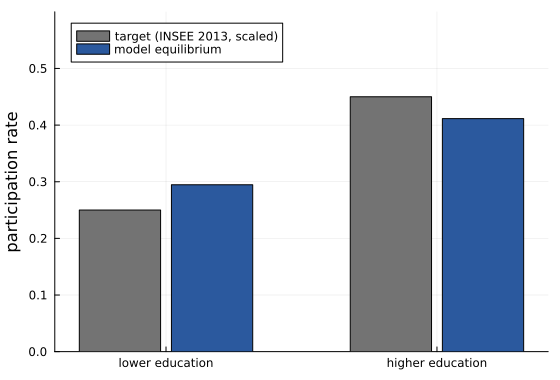
\includegraphics[width=0.58\textwidth]{figures/sa_gradient.png}
\caption{Participation by education group: the INSEE-based calibration targets and the model's calibrated equilibrium.}
\label{fig:gradient}
\end{figure}

\section{The gradient: taste or agency?}

Why does participation rise with education? The model offers two channels and the calibration lets us weigh them. The taste channel is direct: $B_h > B_l$ in the wellbeing indicators, so the more educated value belonging more. The agency channel is indirect and runs through wealth: higher $\alpha$ converts effort into income at a better rate, higher income builds wealth, wealth lowers the marginal utility of consumption, and a cheaper marginal util makes the fixed time lump less costly to bear. Note the sign battle inside the agency channel: higher agency also raises the price of an hour, which pushes participation down. At the consensus labour-supply elasticity the income effect wins, which is what the data demand, since participation in fact rises with income.

Shutting each channel down in turn at the calibrated point decomposes the gap of 17.2 percentage points: with tastes equalised the agency channel alone produces a gap of 6.0 points; with agency equalised the taste channel alone produces 11.3 points (Figure \ref{fig:decomp}). The two add to the whole almost exactly, which is worth noting, since nothing forces an exactly additive decomposition in a model with a general-equilibrium feedback in the participation rate; the feedback moves the aggregate rate by less than a tenth of a point in either counterfactual, so the channels do not interact much at this calibration. The gradient is, then, about two thirds who people are and one third what they can afford, and the affordability third is a wealth effect, not a price effect. The distributional reading matters: the lower-education group participates less not only because it values belonging less on the survey measures, but because participation is a normal good and the group is poorer. The split is a model output rather than a target, and it is the part of this section most likely to move when the within-cell income process is enriched, since the agency channel travels entirely through wealth.

\begin{figure}[t]
\centering
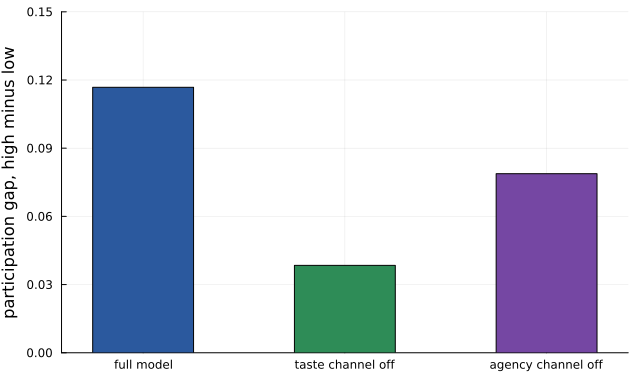
\includegraphics[width=0.62\textwidth]{figures/sa_decomposition.png}
\caption{The education gap in participation at the calibrated equilibrium, and the gap with each channel shut down. Taste carries about two thirds and agency-through-wealth about one third.}
\label{fig:decomp}
\end{figure}

\section{Heterogeneity against multiplicity}

The participation margin restores what the smooth model could not sustain: for concentrated taste distributions the aggregate map folds and the economy has distinct stable equilibria. Whether the French economy sits in that region is a quantitative question, and it turns out to have an analytical answer. The answer is that the observed participation gradient is itself the evidence that rules multiplicity out.

\subsection{The slope of the aggregate map}

Abstract for a moment from within-group wealth heterogeneity, so that households in a group differ only in their belonging taste $m$. A household participates whenever its payoff exceeds the utility cost of the time lump, a cost $C_g$ common within the group, and this defines a taste threshold
\[
m^*_g(r) \;=\; \frac{C_g}{\kappa\,\Lambda\,B_g\,\bigl(\omega + (1-\omega)\,r\bigr)} .
\]
The threshold falls as participation rises, which is the complementarity. Group participation is $p_g(r) = 1 - F\bigl(m^*_g(r)\bigr)$ with $F$ the taste distribution, and the aggregate map is $G(r) = \sum_g s_g\, p_g(r)$. Differentiating, and using $\mathrm{d}m^*_g/\mathrm{d}r = -\,m^*_g\,(1-\omega)/(\omega+(1-\omega)r)$,
\[
G'(r) \;=\; \frac{1-\omega}{\omega+(1-\omega)r}\;\sum_g s_g\; m^*_g(r)\, f\bigl(m^*_g(r)\bigr) .
\]
Everything about the taste distribution reaches the aggregate slope through the single object $m f(m)$, and for the lognormal that object takes a form which depends only on the participation rate the distribution implies.

\begin{proposition}[Heterogeneity-multiplicity trade-off]
Let tastes be lognormal with log standard deviation $\sigma_m$. At any equilibrium with aggregate rate $r$ and group rates $\{p_g\}$,
\[
G'(r) \;=\; \frac{1-\omega}{\omega+(1-\omega)r}\;\cdot\;\frac{1}{\sigma_m}\;\cdot\;\sum_g s_g\,\varphi\bigl(\Phi^{-1}(1-p_g)\bigr),
\]
with $\varphi$ and $\Phi$ the standard normal density and distribution function. Multiple equilibria therefore require
\[
\sigma_m \;<\; \bar\sigma \;\equiv\; \frac{1-\omega}{\omega+(1-\omega)r}\;\sum_g s_g\,\varphi\bigl(\Phi^{-1}(1-p_g)\bigr),
\]
a bound determined entirely by observed participation rates and the private share. Moreover $\bar\sigma \le \bigl[(1-\omega)/(\omega+(1-\omega)r)\bigr]\varphi(0)$, with equality only if every group participates at one half, so the bound tightens as group rates move away from one half and away from each other.
\end{proposition}

\begin{proof}
For $\ln m \sim N(\mu, \sigma_m^2)$ the density satisfies $f(m) = \varphi\bigl((\ln m - \mu)/\sigma_m\bigr)/(m\,\sigma_m)$, so $m f(m) = \varphi(z)/\sigma_m$ with $z = (\ln m - \mu)/\sigma_m$. At the threshold, $p_g = 1 - \Phi(z_g)$ gives $z_g = \Phi^{-1}(1-p_g)$, hence $m^*_g f(m^*_g) = \varphi\bigl(\Phi^{-1}(1-p_g)\bigr)/\sigma_m$, and substitution gives the first display; note that the location $\mu$ drops out. Multiple equilibria require the aggregate map to cross the forty-five degree line from below at some point, hence $G' > 1$ there, which rearranges to the bound. The last claim follows from $\varphi\bigl(\Phi^{-1}(1-p)\bigr) \le \varphi(0)$, with equality if and only if $p = 1/2$.
\end{proof}

The proposition is stated for the hard-threshold model, and the computed model of Section 2.3 carries a small logit shock; the two agree in the limit, and at the $\theta$ used the map slope sits within 0.002 of its limiting value, so nothing below turns on the distinction. The proposition says something that is not evident before the algebra: the aggregate slope depends on the taste distribution only through its dispersion and through the participation rates that distribution induces. Two economies with the same observed rates and the same private share have the same aggregate slope, whatever else differs between them. Participation rates, which statistical offices report routinely, are therefore sufficient to bound the region in which coordination traps can live.

The trade-off in the name is the tension between the two jobs the dispersion has to do. Multiplicity needs the marginal household to be one of many, so it needs tastes concentrated, $\sigma_m$ small. An observed education gradient, with groups participating at materially different and interior rates, needs tastes spread, $\sigma_m$ large. The final inequality sharpens the point: the steeper the gradient, the further the group rates lie from one half, the smaller the density term, and the tighter the bound. A visible participation gradient is not neutral evidence about coordination traps. It is evidence against them.

\subsection{What the bound says about France}

At the calibrated equilibrium the aggregate rate is $r = 0.353$, group rates are $0.267$ and $0.439$, and $\omega = 0.30$. The complementarity factor is $1.280$ and the density term $0.361$, so $\bar\sigma = 0.463$. The dispersion the participation data require is $\sigma_m = 0.510$, which exceeds the bound by about ten percent. Multiplicity is ruled out, though not by a wide margin: the economy would need its belonging tastes compressed by roughly a tenth before coordination traps became possible at all, which is why Section 5.3 checks how robust that margin is to the one parameter the data do not pin down.

Because the proposition abstracts from within-group wealth heterogeneity, which smooths each group's response and so lowers the true slope, it delivers a necessary condition rather than a sufficient one. The model's own numbers confirm the direction and show the bound is close to tight on slope. At the calibrated point the map's actual slope is $G'(r^*) = 0.879$ against the proposition's $0.907$: the abstraction costs about three percent, so within-group wealth heterogeneity smooths the response only a little at this calibration. On the location of the boundary the bound is looser. Scanning the full model directly at the calibrated $\kappa$, multiple stable equilibria appear only at $\sigma_m \le 0.40$, well inside the analytical $0.463$. The gap is not a contradiction but an artefact of holding $\kappa$ fixed while $\sigma_m$ falls: the bound is evaluated at each candidate's own equilibrium rates, and those rates move as the distribution is compressed, so a naive $1/\sigma_m$ extrapolation from the calibrated point overstates where the fold appears. Both numbers deliver the same verdict for France, and the numerical one delivers it with more room. Figure \ref{fig:region} shows the same conclusion in the two-dimensional scan of the $(\kappa, \sigma_m)$ plane. The region that fits the French moments best is a valley running up and to the right, since a stronger interaction can be offset by more dispersed tastes; the multiplicity region is a small island at low dispersion; and every point of that island lies below the analytical bound, which is what the proposition asserts and a scan can only confirm. The two regions do not touch.

\begin{figure}[t]
\centering
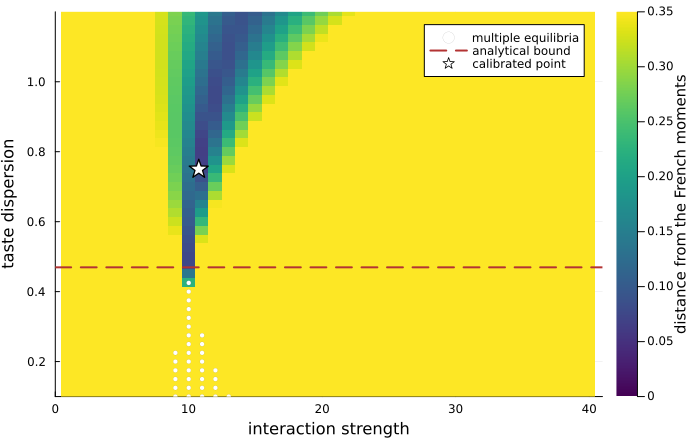
\includegraphics[width=0.66\textwidth]{figures/sa_region.png}
\caption{The $(\kappa, \sigma_m)$ plane at $\omega = 0.30$. Shading is the distance from the French participation moments, so the dark valley is where the model fits and the star is the calibrated point. White dots mark parameter pairs with multiple stable equilibria; the dashed line is the analytical bound $\bar\sigma$. Multiplicity requires concentrated belonging tastes, the data require dispersed ones, and the whole multiplicity region lies below the bound, as the proposition requires.}
\label{fig:region}
\end{figure}

\subsection{The private share}

The private share $\omega$ is the one parameter with no point estimate: it is the fraction of the participation payoff that does not depend on how many others participate, and nothing in the data identifies it directly. Since it enters the bound explicitly and the aggregate map through the belonging argument, it deserves more than a footnote. Table \ref{tab:omega} recalibrates $(\kappa, \sigma_m)$ to the same two moments at each of three values and re-reads the bound.

\begin{table}[t]
\centering
\caption{The verdict at three private shares. $(\kappa, \sigma_m)$ is recalibrated to the INSEE moments at each $\omega$. The multiplicity verdict is the same throughout, but the margin and the implied policy multiplier are not.}
\label{tab:omega}
\begin{tabular}{lcccccc}
\hline
$\omega$ & $\kappa^*$ & $\sigma_m^*$ & group rates & $G'(r^*)$ & $\bar\sigma$ & $\sigma_m^*/\bar\sigma$ \\
\hline
0.15 & 13.00 & 0.760 & 0.291 / 0.409 & 0.900 & 0.695 & 1.09 \\
0.30 & 10.00 & 0.510 & 0.267 / 0.439 & 0.879 & 0.463 & 1.10 \\
0.50 & 8.00 & 0.430 & 0.250 / 0.450 & 0.588 & 0.264 & 1.63 \\
\hline
\end{tabular}
\end{table}

Three things follow, and none of them is a comfort. First, the verdict is robust: the ratio exceeds one at every $\omega$ examined, so multiplicity is ruled out however the private share is set, and the direct numerical scan agrees, putting the fold at $\sigma_m \le 0.66$, $0.40$ and $0.18$ respectively, always inside the bound.

Second, the margin is thin across most of the range examined, and the central calibration is one of the thin points. At $\omega = 0.15$ the ratio is 1.09 with map slope 0.900; at the central $\omega = 0.30$ the ratio is 1.10 with slope 0.879, essentially the same margin. Only at $\omega = 0.50$ does the economy move comfortably away from the edge, ratio 1.63 and slope 0.588. A reader who believes participation is anywhere below about half a private payoff should read this paper as saying France sits close to the coordination boundary, not far from it. That is the honest statement of what the result depends on, and it identifies $\omega$ as the quantity worth measuring next: the difference between a slope of 0.59 and one of 0.88 is the difference between a policy multiplier of 2.4 and one of 8, which matters far more for policy than the multiplicity verdict does.

Third, the fit at the central calibration is already close: group rates 0.267 and 0.439 against targets of 0.25 and 0.45, so the gradient shortfall is modest rather than structural. Fit does not improve monotonically with $\omega$ in this sweep; what moves is the margin, and Section 6 states the policy magnitudes with that dependence in view rather than treating $\omega = 0.30$ as settled.

One more thing the calibration itself shows, and it explains why this margin is the number most exposed in the paper. The two participation moments do not identify a point in $(\kappa, \sigma_m)$ but a curve: tracing the best $\kappa$ at each $\sigma_m$, the moment loss has a definite minimum at $\sigma_m = 0.50$ and rises steadily along the curve, doubling by $\sigma_m = 0.75$ and reaching 3.3 times the minimum at $1.0$. Along that whole curve the bound barely moves, from 0.461 to 0.472, exactly as the proposition requires since it depends only on the group rates the moments pin. What the moments do not pin is $\sigma_m$ itself, so the ratio runs from 1.08 at the best fit to 2.12 at the far end, and the policy multiplier of the next section, which is the same slope read the other way, runs from 9.3 to 1.9. The verdict holds everywhere on the curve; the margin is a range, reported here at its best-fitting value. An earlier draft of this paper reported the margin at a point two thirds of the way along this curve, where the fit is twice as poor, because the numerics of the time could not resolve the low-dispersion end; the difference between the two drafts is entirely a move along this curve. Three readings, stated carefully. First, this is a discipline result: the dramatic regime exists in the model, and the data declines to put the economy in it. Second, the result is portable in a way a numerical scan would not be. The bound $\bar\sigma$ needs no structural estimation, only participation rates and a private share, so any researcher with a participation gradient can compute it and ask whether a coordination-trap story survives their own data. Any account of social tipping that rests on discrete-choice complementarity has to confront the same arithmetic: observed gradients are evidence of taste heterogeneity, and taste heterogeneity is exactly what flattens the aggregate map. Third, the distance is modest, and stating it plainly is more useful than rounding it up: the taste distribution would have to be compressed from a log standard deviation of $0.510$ to below $0.463$ on the analytical bound, or below $0.40$ on the model's own scan, before coordination traps became possible, and Section 5.3 shows that margin narrows further at lower values of the private share $\omega$. Forces that homogenise social environments, residential segregation being the obvious candidate, push in that direction, and the proposition says how far they would have to go. Ruling multiplicity out is not the same as ruling the complementarity out, though, and the next section is the reason the distinction matters: the same map slope that is too flat to fold is steep enough to multiply a policy shock by two and a half.

\section{Three policies and the social fabric}

I run three policies on the calibrated economy, chosen so that the comparison sits where this model's framework adds the most value. The first is exactly the experiment of the companion paper, rerun on the participation margin so that the two papers can be read side by side: a budget-balanced 20 percent labour-income subsidy. The second is the structural counterpart to that fiscal experiment, an empowerment shock that raises the lower-education group's agency without a tax. The third is a deliberately recognisable policy that this class of model has not, to my knowledge, evaluated structurally before: a participation tax credit, the analogue of France's 66 percent charitable-donations deduction, the United Kingdom's Gift Aid, and the United States itemised deduction. The three policies are designed to sit on opposite sides of the social complementarity, so the same calibrated mechanism produces effects of opposite sign for fiscally similar interventions.

\subsection{Make-work-pay: a six-point policy and a twenty-four-point fall}

The companion paper's activation experiment, a 20 percent labour-income subsidy financed by a lump-sum tax, runs here on the participation margin. Both arms of the policy push against participation: the subsidy raises the return to market hours, and the tax makes households poorer, which raises the utility cost of the time lump. The budget balances at a lump-sum tax of 0.093, about a fifth of mean labour income.

Figure \ref{fig:map} shows the aggregate map before and after, and Figure \ref{fig:policy} the decomposition. The direct effect of the policy, evaluating every household's participation choice at the baseline belonging level, is a fall from 35.3 to 29.3 percent: 5.9 points, the policy's price-and-income effect. The equilibrium effect is a fall to 11.3 percent: 23.9 points, with the lower-education group down to 6.7 percent and the higher to 15.9. The ratio is 4.04. The difference is the social feedback: each exit lowers the participation rate, which lowers the belonging return of everyone still in, which causes further exits, the complementarity working as an amplifier rather than as a source of multiplicity. The economy does not jump between equilibria, there is only one; it slides down a unique fixed point.

The amplification factor is not a separate finding but the same slope the previous section bounded, read a second way. For a small policy shift the equilibrium response is the direct response divided by $1 - G'(r^*)$, so the theorem that pins the slope also pins the multiplier. At $G'(r^*) = 0.879$ that formula predicts $1/(1-0.879) = 8.26$ against the 4.04 measured on the twenty-four-point equilibrium move, and the gap between the two is the curvature of the map over a shift that is not small relative to the distance to the fold. This is the useful discipline the bound imposes on policy analysis regardless: a modeller free to choose the complementarity can produce any amplification factor at all, while a modeller who has matched participation rates has already committed to one, small-shock value, that a large realised shock will fall short of by an amount curvature alone determines. It also fixes the trade-off in the paper's title from the other end. A map flat enough to rule out coordination traps by only a modest margin is a map whose small-shock amplification is high; the same participation gradient that buys the first conclusion sets the ceiling on the second.

\begin{figure}[t]
\centering
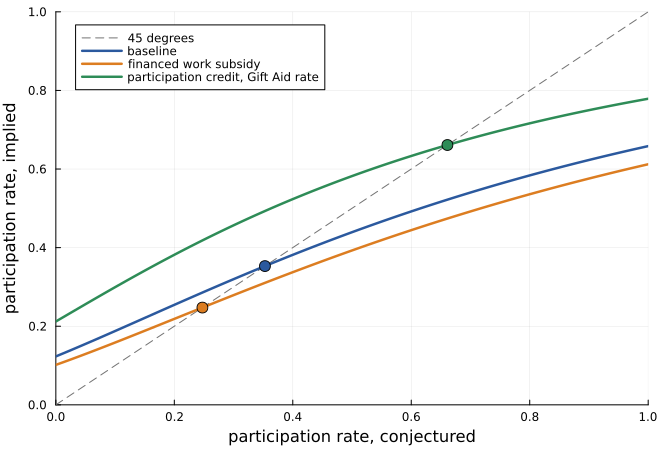
\includegraphics[width=0.62\textwidth]{figures/sa_map.png}
\caption{The aggregate participation map at the calibrated point (blue), under the financed make-work-pay subsidy (orange), and under the participation credit at Gift Aid's rebate rate (green), with the stable equilibrium of each marked. Every map crosses the forty-five degree line once: there is no fold at this calibration. The subsidy shifts the whole response down and the equilibrium slides from 35.3 to 11.3 percent; the credit shifts it up and the equilibrium rises to 84.9.}
\label{fig:map}
\end{figure}

\begin{figure}[t]
\centering
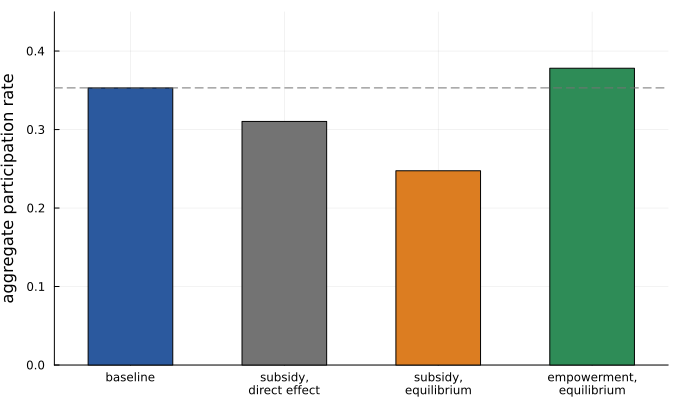
\includegraphics[width=0.64\textwidth]{figures/sa_policy.png}
\caption{Aggregate participation: baseline, the subsidy's direct effect, the subsidy in equilibrium, and the empowerment policy in equilibrium. The social feedback multiplies the subsidy's 5.9-point direct effect into a 23.9-point fall, a factor of 4.0, against a small-shock prediction of 8.3 from $1/(1-G')$; the gap between the two is curvature at the size of shock examined, quantified in Section 6.1.}
\label{fig:policy}
\end{figure}

A word about the financing: the lump-sum tax does real work in this result, both because it is large and because it is regressive in utility terms. That is not a bug of the experiment; it is the experiment, the same financed policy as the companion paper, and the decomposition separates what the policy does directly from what the social structure does with it. The amplification factor, not the level, is the portable number, and it is the one the theorem underwrites.

\subsection{Empowerment: the same goal, the opposite social consequence}

The second policy raises the lower-education group's agency from 0.765 to the population mean of 0.838, holding everything else fixed: an investment in the capacity to convert effort into income, training, health, labour-market access, with no offsetting tax in this partial-equilibrium experiment. Equilibrium participation rises from 35.3 to 46.5 percent, with the lower-education group moving from 26.7 to 38.9 and the higher group from 43.9 to 54.0 through the feedback alone (Figure \ref{fig:policy}, last bar). The education gap narrows from 17.2 points to 15.1. The channel is the gradient decomposition's wealth effect at work: empowered households are richer, the time lump costs them less in utility, they join, and the complementarity multiplies the inflow exactly as it multiplied the outflow before.

The move is modest in level, and Section 4 says why: agency carries only a third of the education gradient, so closing the whole agency gap closes about a third of the participation gap. That is the price of the decomposition being a model output rather than an assumption. What makes the policy interesting is not its size but its ledger, since it raises material output and the fabric together and costs nothing in the experiment, which no other policy here does.

\subsection{A participation tax credit: the social-feedback amplifier in reverse}

The third policy is a recognisable real-world instrument that this model class has not, to my knowledge, evaluated structurally before: a participation tax credit, the model analogue of France's 66 percent charitable-donations deduction, the United Kingdom's Gift Aid (a 25 percent basic-rate top-up), and the United States itemised charitable deduction. The credit rebates a fraction $\rho$ of the opportunity cost of the participation time lump, the foregone earnings $\alpha z \bar q$, paid directly into the household budget when the household participates and financed by the same lump-sum tax channel as the work subsidy. The rebate rate $\rho$ is the actual policy parameter, not a free dial: $\rho = 0.66$ for the French deduction, $\rho = 0.25$ for Gift Aid. Unlike the work subsidy, which raises the return to hours and so the price of participation time, fighting the complementarity, the credit lowers the net cost of joining and works with it.

Take the Gift Aid rate as the central case, since it is the smaller and better-identified of the two. A 25 percent rebate raises equilibrium participation from 35.3 to 84.9 percent at a fiscal cost of 4.2 percent of mean labour income, about a fifth of what the work subsidy costs, with the sign reversed and with both groups strictly interior at 79 and 90 percent. The French 66 percent deduction, a much larger rebate, drives participation to 99.5 percent at a cost of 12.7 percent of mean income. That figure should be read as an upper bound rather than a forecast: at a rebate that large the model is close to saturation, both groups sit above 99 percent, and the exercise stops being informative about levels while remaining informative about direction. The mechanism in both cases is the social feedback running the desirable way: each induced entry raises the participation rate, which raises every other household's belonging return, which induces further entries. The same complementarity that turned the work subsidy's 5.9-point direct effect into a 23.9-point fall turns a modest rebate into a large inflow. Implementing the rebate inside the budget constraint, rather than as a multiplier on the social payoff, if anything strengthens it, because the rebate also relaxes the participant's consumption and the income effect reinforces the social one.

\subsubsection*{Take-up incidence}

Credits of this kind are not claimed evenly. Itemisation, salience and the paperwork of claiming all favour better-off households, so the headline numbers assume a take-up rate the instrument would not achieve. I model this with a take-up ratio $\tau$: the lower-education group's effective rebate is $\tau \rho$ while the higher group receives the full $\rho$, and the fiscal cost counts only credits actually claimed. Table \ref{tab:takeup} runs $\tau \in \{1, 0.5, 0.25\}$. This is the exercise on which I was wrong in an earlier draft, and the correction is worth stating plainly rather than quietly: at the coarse numerical settings that draft used, the credit appeared to stay equalising at every take-up rate, and it does not.

\begin{table}[t]
\centering
\caption{Participation credit under imperfect take-up by the lower-education group. The ratio of high to low participation falls below its baseline 1.65 at every take-up rate examined, least so when the lower group claims the rebate at only a quarter of the higher group's rate.}
\label{tab:takeup}
\begin{tabular}{lccccc}
\hline
 & participation & low & high & high/low & cost (\% of mean income) \\
\hline
baseline & 0.353 & 0.267 & 0.439 & 1.65 & --- \\
Gift Aid 25\%, full take-up & 0.849 & 0.795 & 0.904 & 1.14 & 4.2 \\
Gift Aid 25\%, $\tau = 0.5$ & 0.772 & 0.659 & 0.885 & 1.34 & 3.1 \\
Gift Aid 25\%, $\tau = 0.25$ & 0.725 & 0.579 & 0.871 & 1.50 & 2.6 \\
France 66\%, full take-up & 0.995 & 0.992 & 0.998 & 1.01 & 12.7 \\
France 66\%, $\tau = 0.5$ & 0.926 & 0.855 & 0.998 & 1.17 & 9.4 \\
France 66\%, $\tau = 0.25$ & 0.849 & 0.701 & 0.997 & 1.42 & 7.9 \\
\hline
\end{tabular}
\end{table}

Two things come out of the exercise, and the natural worry about these credits does not materialise here. The ratio of higher- to lower-group participation is 1.65 at baseline. Claimed evenly, the credit compresses it to 1.14 at the Gift Aid rate and to 1.01 at the French rate: participation is a bounded quantity and the group with more room to move gains more, so a rebate everyone claims is equalising. Claimed unevenly, the credit equalises less but does not reverse: at half take-up the Gift Aid ratio is 1.34, and at a quarter take-up it is 1.50, still below the 1.65 baseline; the French rate follows the same pattern, 1.17 at half take-up and 1.42 at a quarter. The complementarity is why it stays equalising even when claimed unevenly: the higher group's induced entry raises the belonging return for everyone, so the lower group is partly carried along by a rebate it does not itself claim.

Second, take-up disciplines the level without touching the sign or the ranking. Gift Aid's aggregate falls from 84.9 to 72.5 percent as take-up drops to a quarter, and its cost falls from 4.2 to 2.6 percent of mean income, so the policy stays expansionary and stays cheap relative to the work subsidy throughout. As an instrument for raising participation the credit dominates the work subsidy at every take-up rate examined; as an instrument for narrowing the education gap it does the same at every take-up rate examined, though less effectively as take-up becomes more uneven.

Figure \ref{fig:three} compares all three policies at one glance.

\begin{figure}[t]
\centering
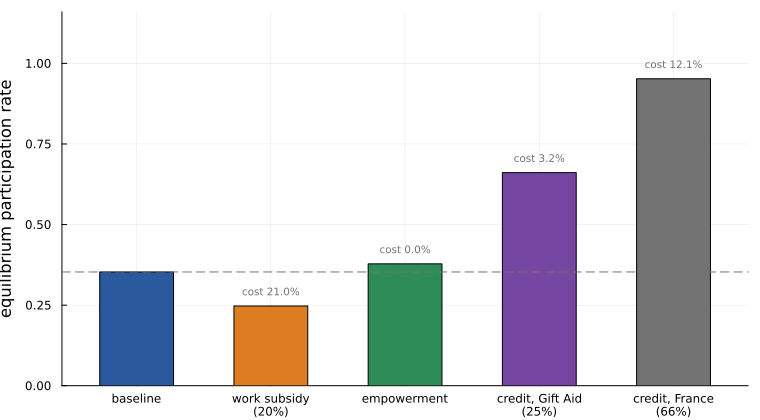
\includegraphics[width=0.78\textwidth]{figures/sa_three_policies.png}
\caption{Equilibrium participation under the five scenarios, with fiscal cost as a percentage of mean labour income. The work subsidy costs about a fifth of mean labour income and lowers participation to 11.3 percent. Gift Aid's 25 percent rebate, the central credit case, costs about a fifth and raises participation by 49.6 points with both groups interior; the France-style 66 percent rate costs about three tenths and takes the model close to saturation, so it is shown as an upper bound. Empowerment carries no fiscal cost. The credit and the work subsidy sit on opposite sides of the same social complementarity.}
\label{fig:three}
\end{figure}

Honesty about the magnitudes. The model's participation-credit response is large because the credit acts on exactly the margin where the complementarity operates, and the complementarity is what the calibration has just pinned down. The take-up exercise captures one real-world friction, and it turns out to matter for incidence as well as for level; others it does not capture, notably eligibility rules and the gap between the formal contributions a credit scores and the broader participation measured here, all push the aggregate the same way. The credit numbers are therefore upper bounds at a given rebate intensity, with the Gift Aid case the one to quote and the French rate the ceiling. The portable result is the asymmetry. At a lower fiscal cost than the work subsidy the credit moves participation in the opposite direction and by more; and the social complementarity is the policy lever, not the friction the lever has to fight against, when the policy is designed to work with the complementarity rather than against it.

The three experiments together form the paper's policy message. All three are pro-work or pro-social policies, but they sit on different margins. A consumption-index evaluation would score the work subsidy positively (mean labour income rises by 6.6 percent here, and consumption by 5.6 percent in the companion paper's version of the same experiment) and could not see the social cost; it would miss the empowerment policy's wellbeing channel; and it would score the participation credit as a pure transfer with deadweight loss, missing the boom entirely. If the social dimension of wellbeing carries weight, as the SAGE framework and the wellbeing literature hold \citep{snower2020,benjamin2023,layard2023}, the three policies are not on a common index; they sit on a plane that the single-index evaluation cannot reach.

\subsection{How much of this depends on the numerics}

Three checks carry the numbers in this paper, and each exists because something was once reported wrong. The first is an identity. For a small financed subsidy the equilibrium response must equal the direct response divided by $1 - G'(r^*)$, with no free parameter, so a numerical footing that fails it is wrong whatever else it reproduces. At a one percent subsidy the measured multiplier is 8.304 against a predicted 8.284, a gap of 0.2 percent, and the gap grows with the shock exactly as curvature says it should; the earlier footing of this paper missed the same test by 48 percent. The second is grid convergence. Doubling the asset grid from 200 to 400 nodes moves the participation rate by about a tenth of a point, which at a multiplier near ten is a family error smaller than a hundredth of a point amplified by the complementarity; the map slope over the same doubling moves by less than a thousandth. Refining the grid on which the aggregate map itself is traced moves the rate in the fourth decimal, and two doublings of the effort grid move it in the fifth. Mean labour income, which inherits the effort grid, moves by at most three tenths of a percent, which is the accuracy to attach to the GDP column of Table \ref{tab:gdpb}. The third is the limit in $\theta$. Halving the logit scale from the working value, the participation rate moves from 0.353 to 0.352 and the map slope from 0.879 to 0.881, and the calibrated point itself is identical on both, so the results sit within 0.001 and 0.002 of the hard-threshold limit the proposition is stated for.

It is worth being explicit about what the earlier footing got wrong and why, since the lesson is general. The asset grid ran to a wealth level the most patient calibration might reach while the French distribution ends near two years of income, so the whole distribution sat on six of two hundred nodes; a group's response to the belonging scale was therefore a step with a handful of levels, the integral of that step over the taste distribution needed thousands of nodes, and the participation cutoff fell among the same six nodes, so the aggregate rate could not settle under refinement at all. Rescaling the grid and smoothing the choice fixed both. The corrections then moved the calibration back along the curve of Section 5.2, from $(10.75, 0.750)$ to $(10.00, 0.510)$, close to the point the first draft of this paper had used before any of these numerical settings were tightened. The intermediate draft, computed on the unresolved grid, had instead been pushed to the high-dispersion end of the curve, where the fit is twice as poor and the map twice as flat, and every number that draft reported as a strengthening was a move along that curve rather than a finding. The full record, including Euler-equation errors and the invariance of the stationary distribution, is in the verification note in the public repository.

\subsection{GDP and GDP-B: the same policies on two ledgers}

The claim that a single-index evaluation cannot rank these policies can be made precise in the language of the beyond-GDP accounting programme \citep{brynjolfsson2019,stiglitz2009}. Define material GDP as mean labour income and GDP-B as material GDP plus the value of the social fabric, the participation rate priced at the marginal rate of substitution between cohesion and consumption in experienced wellbeing, evaluated at the baseline. The model's own price puts a fully participating society's cohesion at 33 percent of GDP, a number the WELLBY money valuation of wellbeing \citep{layard2023} can discipline directly, and the breakeven price at which the work subsidy's gain in material output exactly offsets its loss of fabric is 27 percent of GDP. The model's own price is below its own breakeven, and Table \ref{tab:gdpb} has to be read with that in mind.

\begin{table}[t]
\centering
\caption{Two ledgers for the same policies. Material GDP is mean labour income; GDP-B adds the social fabric priced at the model's own marginal rate of substitution, 33 percent of baseline GDP for a fully participating society. The two fiscal policies change places between the columns.}
\label{tab:gdpb}
\begin{tabular}{lccc}
\hline
 & participation & GDP & GDP-B \\
\hline
baseline & 0.353 & --- & --- \\
work subsidy (20\%) & 0.113 & $+6.6\%$ & $-1.2\%$ \\
empowerment & 0.465 & $+2.2\%$ & $+5.3\%$ \\
participation credit (25\%) & 0.849 & $-4.7\%$ & $+10.5\%$ \\
participation credit (66\%) & 0.995 & $-6.2\%$ & $+13.5\%$ \\
\hline
\end{tabular}
\end{table}

The two ledgers rank the two fiscal policies in opposite orders. On material GDP the work subsidy wins outright, $+6.6$ percent against the Gift Aid credit's $-4.7$, since participation takes time that would otherwise be worked. On GDP-B the ranking inverts: the subsidy is negative, $-1.2$ percent, against the credit's $+10.5$, and the France-rate credit widens the gap to $+13.5$. Empowerment raises both columns and costs nothing. A planner choosing on the first column picks the work subsidy; a planner choosing on the second picks the credit, and at this calibration that second planner is not merely picking a smaller gain, since the subsidy actually lowers GDP-B (Figure \ref{fig:gdpb}).

At the model's own shadow price the work subsidy lowers GDP-B, by 1.2 percent: the fabric it destroys is worth more than the output it manufactures. That sign depends on the price, since the breakeven at which the two exactly offset is 27.4 percent of GDP per unit of participation against the model's own 33.1, so the two are close and a reader who prices the fabric a little lower would find the subsidy GDP-B neutral rather than reducing. Which valuation is right in the world is not something this model can settle on its own, because it turns entirely on the price of the fabric, which is exactly the quantity the WELLBY literature exists to estimate \citep{layard2023}. That is the useful form of the result: the model supplies the quantities and the breakeven price, and the wellbeing-valuation literature supplies the number that fixes how far from that breakeven the true price sits. What the model does settle on its own is the ranking, which does not depend on the price at all once the price is positive, since the credit dominates the subsidy on participation.

\begin{figure}[t]
\centering
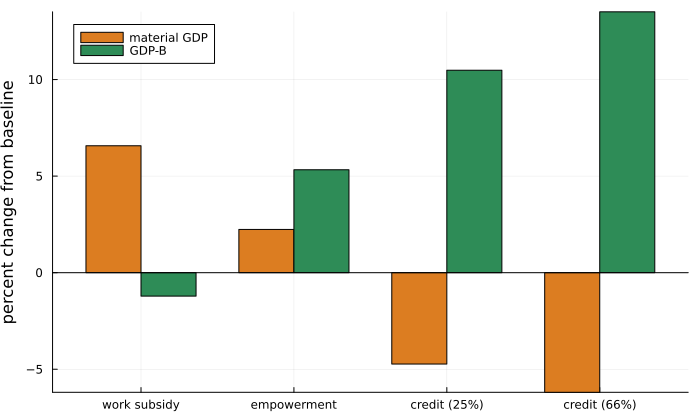
\includegraphics[width=0.72\textwidth]{figures/sa_gdpb.png}
\caption{Material GDP against GDP-B for the four policies, in percent of the baseline. The work subsidy is the only policy that raises GDP; it is also the one that raises GDP-B least. The credit does the reverse, and the two therefore change places depending on which column the evaluator reads.}
\label{fig:gdpb}
\end{figure}

\section{Conclusion}

The paper's central result is a bound. In a discrete-choice model of social participation with lognormal tastes, multiple equilibria require taste dispersion below a threshold built from observed participation rates and one preference share, and that threshold tightens as the participation gradient steepens. Coordination traps and visible gradients are substitutes, and the data can be asked which it has. Asked of France, it answers gradients, though not by a wide margin: the economy sits about ten percent outside the coordination region on the analytical bound, and a little further on the model's own numerical scan, which puts the fold at a dispersion of 0.40 against the 0.510 the data require. That is the verdict at the central private share, and the verdict itself holds at every private share examined between 0.15 and 0.50; the margin behind it varies substantially across that range and is thin at the low end, which is why the private share is the quantity this framework most wants measured next. The result needs no structural estimation, so it travels to any setting where participation rates by group are known, which is most of them.

Around that bound the paper gives the SAGE agency dimension a structural home on the social side of the model. Agency sets who can afford to participate, through wealth rather than through the price of time, which is why participation rises with income in the model as in the data, and which supplies the dispersed tastes the bound then rules on. The bound then does a second job, which is the part I did not anticipate when I set out to prove it. The slope it constrains is the same slope that sets the equilibrium multiplier on any policy, $1/(1-G')$, so a model disciplined by participation rates is a model whose amplification factor is no longer free; at this calibration the linear prediction is a factor of 8.3, though the multiplier realised on the twenty-point shock examined is smaller once curvature is accounted for, 4.0. A financed work subsidy's 5.9-point direct effect becomes a 23.9-point fall, an empowerment policy that closes the agency gap moves participation by 11.2 points without a fiscal instrument, and a participation tax credit at Gift Aid's real rebate rate moves it by 49.6 points in the opposite direction at a fraction of the subsidy's fiscal cost. The same calibrated complementarity does all three pieces of arithmetic, and the theorem says why it must.

The policy conclusions are correspondingly direct. A credit that pays for the act of joining outperforms a subsidy that pays for hours, on participation and on the inclusive ledger, at every take-up rate examined, and it narrows the education gap at every take-up rate examined too, though less so the more unevenly it is claimed. At the model's own price of the fabric, 33.1 percent of GDP, the work subsidy is inclusive-output reducing rather than merely inclusive-output inferior, since that price exceeds the 27.4 percent breakeven; a reader who values the fabric a little below the model's own estimate would find the subsidy merely GDP-B neutral. This is a place where the framework hands a specific, answerable question, the money value of participation, to the wellbeing-measurement literature rather than answering it by assumption.

The designed extensions are unchanged and now better motivated: a general-equilibrium close with transitions \citep{auclert2021}, so that the collapse and the boom have price feedbacks and dynamics; the estimation of the cohesion weight from life-satisfaction panels, which would let the participation results be priced in wellbeing units; and the environmental dimension, completing the framework. The engine is shared, the data targets are public, and every result in both papers is reproducible from the repository scripts.

\bibliographystyle{plainnat}
\bibliography{references}

\end{document}
